\documentclass[12pt]{article}
\usepackage{amsmath}
\usepackage{amssymb}
\usepackage{latexsym}
\usepackage{graphicx}
\usepackage{mathrsfs}
\usepackage{CJKutf8}
\author{qit}
\title{暑期培训——网络编程基本介绍}
\begin{document}
\begin{CJK}{UTF8}{gbsn}
\maketitle

\section{分层协议}
\subsection{协议栈}
\begin{tabular}{lr}
\hline
1&应用层\\ 
\hline
2&运输层\\
\hline
3&网络层\\
\hline
4&链路层\\
\hline
5&物理层\\
\hline
\end{tabular}

\subsection{各层简介}
\subsubsection{应用层}
\paragraph{}应用层指的是网络应用程序和他们之间的通信协议。
\paragraph{}e.g. 浏览器和服务器上部署的相应的软件就都是网络应用程序,属于协议层。同时,他们之间"通信的协议",即浏览器如何给服务器发送请求和服务器如何给浏览器返回相应的html文本及其他资源的协议,应用层协议:HTTP。

\subsubsection{运输层}
\paragraph{}运输层提供了在应用程序的端点之间传送应用层报文的服务,即将进程发送来的报文在首部加上一定的附加信息传递形成报文段,并向下传递给网络层。
\paragraph{}因特网常用的运输层协议为TCP和UDP,单独介绍。

\subsubsection{网络层}
\paragraph{}网络层将从运输层得到的报文段和目的地址发送给我们的目的端的主机,网络层中的一块数据称为数据报。
\paragraph{}包含两个协议,IP协议和选路协议。IP协议是让路由器明白如何作用于数据报中的各个字段,选路协议是规定了数据报从源传送到目的地所走的链路。

\subsubsection{链路层}
\paragraph{}在一系列packet交换机(路由器,链路交换机)之间发送我们的packet。

\subsubsection{物理层}
\paragraph{}在一系列packet交换机(路由器,链路交换机)之间发送我们的packet,同时与链路的实际传输介质相关(同轴线、光纤等)。

\subsubsection{整体结构}
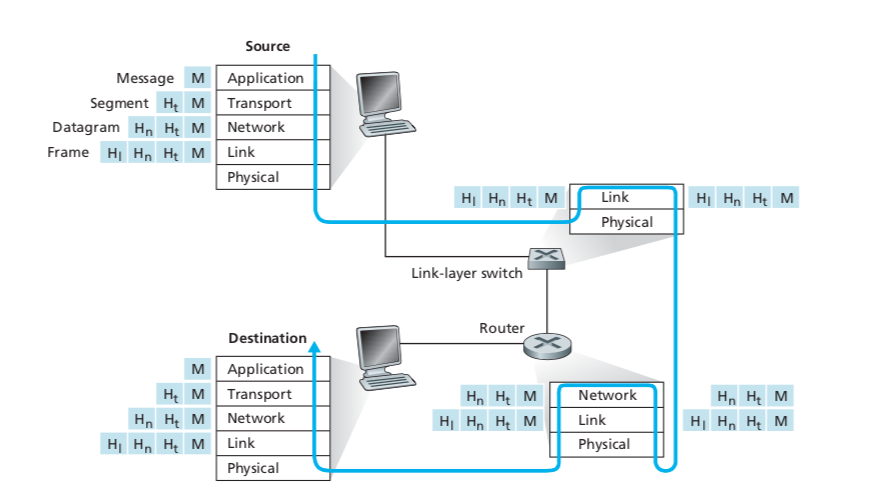
\includegraphics[width=7in]{arch.png}

\subsubsection{ts20中我们需要掌握的}
\paragraph{应用层  进程间通信}
\paragraph{应用层和运输层之间的API  socket}
\paragraph{传输层协议的了解  TCP/UDP}

\section{TCP/UDP}
\subsection{C/S}
\paragraph{C/S结构}Client/Server结构,是指有一个主机(进程)充当服务器,他总是打开,并监听来其他进程的连接申请。其他和该主机(进程)建立连接的进程称为Client。在C/S结构下,client之间不互相通信。
\paragraph{}ts中,使用C/S的编程模式。

\subsection{TCP}
\paragraph{1.}首先使用TCP运输协议的两个进程之间会先建立一个链接,这个链接经过3次握手之后建立完成。\\
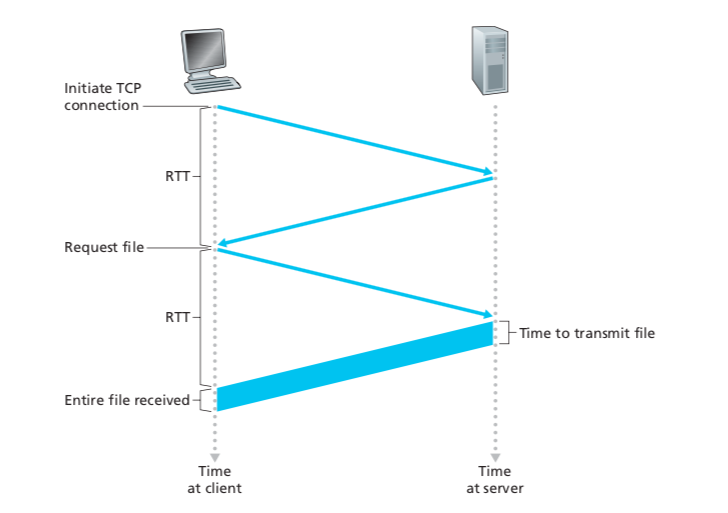
\includegraphics[width=6in]{handshake.png}
\paragraph{2.}之后在两个进程之间发送数据,具有保证不丢失数据(如果丢失数据,会要求更底层重新发送)的特点。但代价是传输速率没有保证。

\subsection{UDP}
\paragraph{1.}使用UDP协议的两个进程之间不需要建立连接,直接互相发送数据。
\paragraph{2.}不保证数据一定会送达,但是传输速率较快。

\section{socket}
\subsection{进程间寻址}
\paragraph{}在网络编程中,两个进程如果相互发送数据,那么就应该知道另一个进程的“地址”。这个地址首先是这个进程运行在哪一台主机,主机是用IP进行标识的,“可以认为”IP地址是唯一标识一台主机的32位比特数。
\paragraph{}其次,在知道了主机地址之后,我们还应该知道应该发给主机的哪一个进程,这个进程是用端口号进行标识的。
\paragraph{}端口号的范围是0-65535,同时较小的端口号可能会被操作系统中的一些进程占用。一般使用>1024的端口号就不会出现什么问题。
\paragraph{}本地主机的IP为127.0.0.1。
\subsection{socket概念}
\paragraph{}socket是一个抽象概念,指的是应用层和协议层之间的一套软件接口API,让我们在应用层中的写的软件程序能够和运输层解耦。
\subsection{python下socket实现TCP通信}
\paragraph{1.}import socket
\paragraph{2.}server=socket.socket(socket.AF\_INET,socket.SOCK\_STREAM)。 \\实例化一个socket
\\其中socket.AF\_INET表明我们使用IPV4协议,如果使用IPV6协议进行通信,则应该指定为socket.AF\_INET6。
\\socket.SOCK\_STREAM是指定运输层协议我们使用TCP协议。
\\此时我们就建立好了一个使用TCP运输协议的socket,也基本完成了我们对运输层及以下层的设置。
\paragraph{3.}server.bind((IP,port))
\\是C/S编程中server做的监听对应IP的对应端口port操作,之后这个server进程就会监听这个端口号,等待client发送来的链接请求。
\paragraph{4.}server.listen(number)
\\是server能够连接的最多的client的数目。
\paragraph{5.}client.connect((IP,port)) 
\\是C/S编程中client应该发出的链接请求,其中IP是服务器的IP号,port是服务器上正在运行的对应进程正在监听的端口号。
\paragraph{6.}sock,addr=server.accept()
\\是C/S编程中server作出的接受链接的指令,接受链接后,会返回一个对应的sock客户端链接和客户端链接地址addr。
\paragraph{7.}number=sock.send(bitstream)
\\向链接的另一端的进程发送一个bitstream,其中返回值number是发送了的比特数。
\paragraph{8.}sock.recv(bitnumber)
\\从链接的另一端的进程接受一个长度不超过bitnumber的一个bitstream。

\subsection{python下socket实现UDP通信}
\paragraph{1.}import socket
\paragraph{2.}sock=socket.socket(socket.AF\_INET,socket.SOCK\_DGRAM)。 \\实例化一个socket
\\其中socket.SOCK\_DGRAM指的是使用UDP运输协议。
\\注意,由于UDP协议下,不会建立连接,因此不会有listen、accept等方法。
\paragraph{3.}sock.bind((IP,port))
\\实例化的sock绑定对应的IP和端口号。
\paragraph{4.}data,addr=sock.recvfrom(number)
\\接受发送到当前进程绑定的端口的数据,接受到的bitstream长度不超过number。
\\返回值为data即发送来的bitstream和addr即发送方的IP和port
\paragraph{5.}number=sock.sendto(bitstream,(IP,port))
\\把bitstream发送给绑定了对应IP和port的进程,同时对方会收到当前发送进程的IP和port,如果没有自己绑定port,操作系统会自动为当前进程绑定一个port。
\\返回值number为成功发送的bit数目。

\section{应用层}
\subsection{进程间通信}
\paragraph{1.}由于在ts中,一般采用C/S模式编程,因此有1个server和两个client。server下一般是使用一个主线程和两个监听线程,会涉及到进程/线程间通信的问题。最为重要,下一次课单独讲解。
\subsection{应用层的通信格式}
\paragraph{1.}应用层互相发送的都是bitstream,因此应该互相约定通信格式,以便彼此能从收到的bitsream中decode出有用的信息。
\paragraph{2.}使用protobuf库进行序列化。

\section{现场演示socket编程}

\section{参考资料}
\paragraph{1.}计算机网络 自顶向下方法
\paragraph{2.}https://www.liaoxuefeng.com/wiki/0014316089557264a6b348958f449949df42a6d3a2e542c000




\end{CJK}
\end{document}
